\documentclass[12pt]{article}

\usepackage{sbc-template}

\usepackage{graphicx,url}

%\usepackage[brazil]{babel}   
\usepackage[utf8]{inputenc}  
     
\sloppy

\title{NOSQL - Armazenamento e Recuperação de dados não-relacional}

\author{Bruno Santos de Lima\inst{1}, Leandro Ungari Cayres\inst{1} }


\address{Faculdade de Ciências e Tecnologia\\
  Universidade Estadual Paulista \\
  "Júlio de Mesquita Filho" \\
  Caixa Postal 19060-900  -- Presidente Prudente -- SP -- Brasil
  \email{brunoslima4@gmail.com, leandroungari@gmail.com}
}

\begin{document} 

\maketitle

\begin{abstract}
Traduzir o resumo...
\end{abstract}
     
\begin{resumo} 
Fazer... (última coisa)
\end{resumo}


\section{Introdução}
\label{sec:intro}
Irrefutavelmente, é possível notar o crescimento da tecnologia com isso o número de dispositivos eletrônicos, sejam eles supercomputadores, computadores desktop ou aplicações moveis, vem aumento em grandes proporções tornando-se presentes nas mais variadas situações do dia a dia, cada qual buscando manipulando diversos dados referentes ao contexto em que eles são aplicados, seja no âmbito empresarial, hospitalar, juridico, academico e diversos outros setores.

Com as diversas aplicações e diversos dispositivos atuando diariamente na vida da sociedade no que diz respeito a manipulação de dados, surge a necessidade de realizar inicialmente o armazenamento desses dados afim de poder manipula-los de forma eficiente e segura para abstrair informações relevantes sobre determinado contexto onde esses dados estão inseridos e com isso facilitar, ajudando a sociedade a utilizar essas informações para realizar algumas atividades diarias, o responsavel por realizar esse armazenamento e conseguentemente a manipulação desses dados é o chamado Banco de dados.

Quando o assunto Banco de dados é abordado logo é pensado como os dados não armazenados e manipulados? para isso é seguido um modelo, de certa forma uma padronização, para responder esta pergunta, o modelo mais conhecido e utilizado em larga escala por Sistemas Gerenciadores de Banco de Dados (SGBD's) é denominado modelo relacional \cite{codd:1970} criado por Edgar Frank Codd em 1970, o modelo relacional substituiu o modelo anterior chamado de modelo hierarquico tornando-se um padrão referencia para este quesito, sendo utilizado pela grande maioria dos SGBD's, onde podemos citar por exemplo os mais conhecidos atualmente: MySQL, Oracle, SQL Server e PostgreSQL.\cite{brito2010bancos}

Contudo atualmente o modelo relacional produz a flexibilidade que o cenario atual exirge e vem sendo substituido em algumas areas pelos chamados NoSQL, este artigo tem como foco abordar o modelo NoSQL apresentando suas caracteristicas, formas de armazenamento e recuperação dos dados e alguns contrastes ao modelo relacional.

Este artigo esta organizado como segue: na seção \ref{sec:nosql}.....

%melhorar e acrescentar bem mais....

\section{NOSQL} 
\label{sec:nosql}

Com o decorrer do tempo foi pensado em modelagens alternativas ao tão utilizado modelo relacional, tais pensamentos justificam-se devido a algumas limitações presente no modelo relacional, limitações essas relacionadas a falta de flexibilidade fornecida pelo modelo relacional.

O NoSQL foi idealizado em 1998 e tem como significado de seu termo "não somente SQL", pois a ideia é que ambos os modelos, tanto o relacional quanto o NoSQL, possam coexistir, cada um em seu espaço de atuação, ou seja, existem aplicações em que o modelo relacional é mais interessante de se utilizar, porem também existem aplicações em que o NoSQL é mais viavel, por exemplo em aplicações distribuidas, onde o armazenamento dos dados é distribuido, sendo esses dados de grande escala, como por exemplo redes sociais tais como Facebook e Twitter e podem acumular Terabits de dados todos os dias, não existindo um esquema fixo, assim para este tipo de aplicação o NoSQL é mais vantajoso.\cite{gueidi:2016} 

Os Banco de dados NoSQL fornecem mecanismos de aramzenamento e recuperação de dados que são modelados como não estruturado, diferente da forma disposta por tabelas utilizada pelos Banco de dados Relacionais \cite{zhaoSchema:2014}, sendo assim o NoSQL não é relacional, essa seria a principal caracteristica do NoSQL, porem seu conceito é muito amplo podendo existir banco de dados NoSQL com algumas caracteristicas diferentes de outros banco de dados NoSQL, isso deve-se a flexibilidade que ele prove, entretando existem um grupo de caracteristicas comuns entre os banco de dados NoSQL, tais caracteristicas são descritas abaixo:

\begin{itemize}
	\item Distribuido: O banco de dados NoSQL são em geral distribuidos, assim varias maquinas são resposaveis por armazenar e prover esses dados quando os mesmos forem requisitados.\\
	\item Escalabilidade horizontal:  \\
	\item Grande volume de dados: Um dos propositos do NoSQL é ter a capacidade de armazenar uma grande quantidade de dados de modo mais rapido possivel.\\
	\item SQL não é suportado: De uma modo geral nos Banco de dados NoSQL não é utilizado a linguagem SQL, assim cada sistema tem seu proprio modo de realizar consultas, existem estudos e também já existe uma alternativa proposta de unificar as consultas em Banco de dados NoSQL.\\
	\item Base: \\
\end{itemize}

\section{Categorização dos Banco de dados NOSQL}
\label{sec:categorizacao}

O NOSQL pode ser classificado em cinco categorias \cite{typeNOSQL:2013} sendo elas: Banco de dados de armazenamento chave-valor, Banco de dados orientado por colunas, Banco de dados orientado a documentos, Banco de Dados orientado a grafos e Banco de Dados orientado a objetos.

Em Banco de dados de armazenamento chave-valor os dados tem duas informações associadas a ele, uma sendo a chave e a outra sendo o valor, onde esse valor é literalmente o dado armazenado, como isso seu mecanismo de funcionamento atua de forma similar a um hash, trazendo como um aspecto positivo a rapidez em sua manipulação, não só isso mas também alta concorrência e armazenamento em massa, porem o grande ponto negativo deve-se a falta de uma esquematização o que deixa a visualização da organização desses dados dificultada.\cite{typeNOSQL:2013}

Em Banco de dados orientado por coluna consiste em uma organização onde o dados não são armazenados em linhas mas sim em colunas, ou seja, ocorre uma mudança de orientação agora sendo por atributos, colunas, e não mais por registros, tuplas. Dois exemplos dessa categoria de Banco de dados orientado por colunas é o Cassandra e o BigTable.\cite{brito2010bancos}\cite{surveyNosql:2012}

Em Banco de dados orientado a documentos os dados são armazenados na forma de documentos que tem uma chave unica associada a ele, essa chave é uma string que representa o caminho, ou URI, onde o documento está armazenado, no geral é fonecido uma API ou uma linguagem de consulta para que esses documentos possam ser recuperados rapidamente. \cite{surveyNosql:2012} Uma vantagem relacionado a essa categoria está no aproveitamento de espaço de armazenamento, visto que um documento tem um tamanho necessario para armazenar os dados em que nele estão sem que ocorra desperdicio de espaço, já no modelo relacional os dados são armazenados em tabelas sendo que alguns campos dessa tabela podem ficar vazios disperdiçando espaço, um exemplo de SGBD que utiliza este modelo o MongoDB. Esse modelo deve ser evitado em aplicações que envolvem muitos relacionamentos.\cite{typeNOSQL:2013}

Em Banco de dados orientado a grafos armazenam os dados na forma de um grafo, sendo que cada nó é um objeto e o relacionamento entre esses objetos é expresso pelas arestas que ligam dois nós. Esse tipo de modelo é indicado para redes sociais, sistemas bioinformatica entre outros, pois os nós podem representar por exemplo pessoas ou negocios semelhantes aos objetos utilizados em determinadas linguagens de programação, entretanto apresenta um desvantagem pois é dificil realizar um agrupamento desses dados.\cite{typeNOSQL:2013}\cite{surveyNosql:2012} 

Em Banco de dados orientado a objetos os dados são armazenados na forma de objetos, objetos analogos aos do paradigma de programação orientado a objetos oferecendo recursos como encapsulamento, polimorfismo e herança, cada objeto tem um idenficador unico que representa o objeto unicamente.\cite{typeNOSQL:2013}

\section{Sistemas Gerenciadores de Banco de Dados Não relacionais}

\section{Banco de dados: relacional vs não relacional}

\section{NoSQL: Vantagens e desvantagens}
\label{sec:vantagensedesvantagens}

Como toda tecnologia o NoSQL também apresenta um conjunto vantagens e desvantagens em sua utilização, é importante acrescentar que essas vantagens e desvantagens em sua utilização pode sofrer varianças de acordo com a necessidade de uma aplicação ou organização, ou seja, dependendo do proposito da aplicação as desvantagens são minimizadas devido a grande parcela de beneficios. A seguir é discutido algumas vantagens e desvantagens em sua utilização.

\subsection{Vantagens}
\label{subsec:vantagens}

Os Bancos de dados NoSQL tem como sua grande vantagem o processamento mais rapido dos dados que estão armazenados se comparado com os Bancos de dados Relacionais. O fator que torna o Banco de dados relacional mais lento em processamento é caracterizado pelas chamadas restrições ACID, cujo a sigla representa Atomicidade, cosistência, isolamento e durabilidade. 

Atomicidade significa que toda atualização é executada por completa ou não, já a consistência é o fato de toda transação estar proibida de quebrar as regras do banco de dados, isolamento deve-se ao fato de que cada aplicação faça transações de modo independente a outras aplicações que estão atuando em paralelo. Essas restrições são importantes no quesito precisão, porem se utilizadas causam uma perda de desempenho no processamento, o NoSQL não utiliza o suporte para as restrições ACID aumentando o seu desempenho de processamento.\cite{leavitt:2010}

A não utilização das restrições ACID não torna o NoSQL um Banco de dados inconsistente ou inseguro, apenas diminui essas capacidades, porem não as elimina por completo devido a utilização da BASE como uma alternativa ao conjunto ACID.\cite{pritchett:2008}

Um outro aspecto para o processamento mais rapido de dados nos Bancos de Dados NoSQL é a simplificação do modelo, ou seja, de um modo geral seus modelos são mais simples facilitando seu processamento. Outra vantagem interessante do NoSQL está na flexibilidade que o modelo prove, essa flexibilidade permite que as organizações e desenvolvedores utilizem seus aplicativos da forma que melhor atenda suas necessidades.\cite{leavitt:2010}

\subsection{desvantagens}
\label{subsec:desvantagens}

O NoSQL apresenta ainda alguns desafios, sendo um deles a maior complexidade devido a não utilização de SQL, todos as consultas devem ser realizadas manualmente através da programação, esse fator pode não ser um problema em consultas simples, porem podem potencializar um problema para as tarefas mais dificeis. A falta de ferramentas para gerenciamento ou mesmo para utilização como suporte parte do cliente ainda é um problema, onde essa falta de ferramentas pode estar relacionado ainda ao desconhecimento da tecnologia que pode ser um outro problema.\cite{leavitt:2010}

Devido a não utilização de restrições ACID quesitos como confiabilidade e a consitência tornam-se um problema em Banco de dados NoSQL sendo uma desvantagem, principalmente para certos tipos de aplicações como bancarias este modelo não é recomendado.\cite{leavitt:2010}

\section{Armazenamento e recuperação em banco de dados não relacional}


%\subsection{Subsections}


%\section{Figures and Captions}\label{sec:figs}


%\begin{figure}[ht]
%\centering
%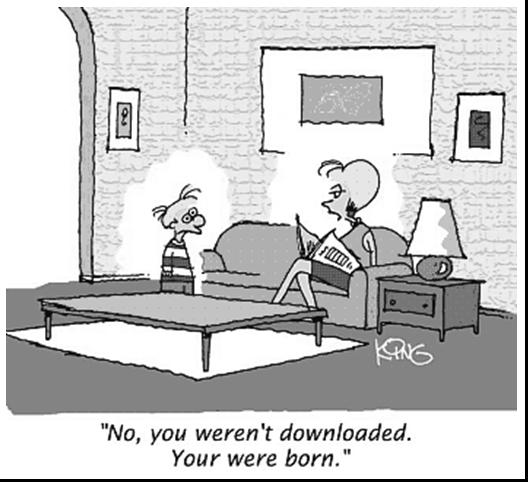
\includegraphics[width=.5\textwidth]{fig1.jpg}
%\caption{A typical figure}
%\label{fig:exampleFig1}
%\end{figure}

%\begin{figure}[ht]
%\centering
%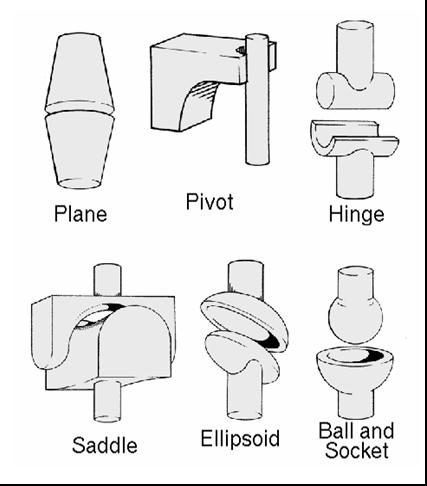
\includegraphics[width=.3\textwidth]{fig2.jpg}
%\caption{This figure is an example of a figure caption taking more than one
%  line and justified considering margins mentioned in Section~\ref{sec:figs}.}
%\label{fig:exampleFig2}
%\end{figure}

%\begin{table}[ht]
%\centering
%\caption{Variables to be considered on the evaluation of interaction
%  techniques}
%\label{tab:exTable1}
%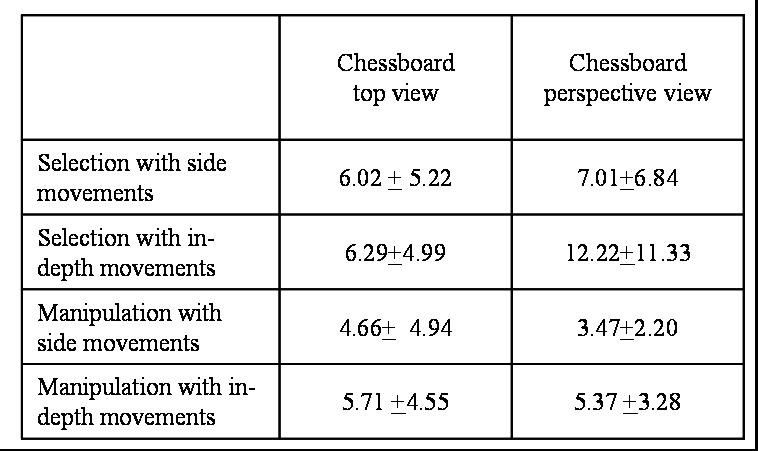
\includegraphics[width=.7\textwidth]{table.jpg}
%\end{table}

\section{Conclusão}
\label{sec:conclusao}

\bibliographystyle{sbc}
\bibliography{sbc-template}

\end{document}
